\documentclass{article}
\usepackage[utf8]{inputenc}
\usepackage{amsmath,amsfonts,graphicx}
\usepackage{algorithm,caption}
\usepackage[noend]{algpseudocode}
\usepackage{float}
\usepackage{tikz}
\usepackage{hyperref}
\hypersetup{
    colorlinks   = true, %Colors links instead of surrounding boxes
    urlcolor     = magenta, %Color for external hyperlinks
    linkcolor    = blue, %Color of internal links
    citecolor   = magenta, %Color of citations
    filecolor = cyan,      
}

\algnewcommand\algorithmicinput{\textbf{Input:}}
\algnewcommand\INPUT{\item[\algorithmicinput]}

\algnewcommand\algorithmicoutput{\textbf{Output:}}
\algnewcommand\OUTPUT{\item[\algorithmicoutput]}

% use these for theorems, lemmas, proofs, etc.
\newtheorem{theorem}{Theorem}
\newtheorem{lemma}[theorem]{Lemma}
\newtheorem{proposition}[theorem]{Proposition}
\newtheorem{claim}[theorem]{Claim}
\newtheorem{corollary}[theorem]{Corollary}
\newtheorem{definition}[theorem]{Definition}
\newenvironment{proof}{{\bf Proof:}}{\hfill\rule{2mm}{2mm}}

\title{Feedback Arc Set}
\author{Anurag Uppuluri}
\date{May 2020}

\begin{document}

\maketitle

\section{Problem Definition}
Given a digraph\footnote{could also be edgeless}, $G = (V,E)$, a {\em feedback arc set} (FAS) or {\em feedback edge set} is a set of edges, $S\subseteq E$, such that every directed cycle in $G$ has at least one edge in $S$. In other words, removing $S$ from $G$ would remove all the cycles in $G$ and make it a Directed Acyclic Graph (DAG).~\cite{noauthor_feedback_2020}

For example, in the following graph (figure~\ref{fig:my_label}), all possible directed cycles are:

\begin{itemize}
    \item $g-f-c-d-g$\footnote{where `$-$' represents an edge}
    \item $f-c-d-e-f$
    \item $f-d-e-f$
    \item $c-g-f-c$
    \item $c-d-e-c$
    \item $d-g-e-f-d$
    \item $d-g-e-f-c-d$
    \item $d-g-e-c-d$
    \item $d-g-f-d$
\end{itemize}

And, some possible feedback arc sets might be:

\begin{itemize}
    \item $S = \{(b,g), (g,f), (f,c), (c,g), (e,c), (d,e), (d,g)\}$
    \item $S = \{(b,g), (g,f), (f,c), (c,g), (e,c), (d,e)\}$
    \item $S = \{(g,f), (f,c), (c,g), (e,c), (d,e), (d,g)\}$
    \item $S = \{(g,f), (f,c), (c,g), (e,c), (d,e), (g,e)\}$    
\end{itemize}

\begin{figure}[H]
    \centering
    \includegraphics[scale=0.8]{figures/feedback-arc-set.png}
    \caption{Finding Feedback Arc Sets}
    \label{fig:my_label}
\end{figure}

We would say that the feedback arc set $\{(b,g), (g,f), ( f,c), (c,g), (e,c), (d,e), (d,g)\}$ has {\em size} 6, and the feedback arc set $\{(g,f), (f,c), (c,g), (e,c), (d,e), (g,e)\}$ has size 5. A trivial feedback arc set for any graph $G$ would be obtained by including all the edges of $G$ in it. We are more interested in finding the smallest feedback arc set:

\vspace{.5cm}
\noindent\fbox{
\parbox{\textwidth}{
{\bf Feedback Arc Set}

    {\bf Input:} A graph $G = (V,E)$

    {\bf Goal:} Return a feedback arc set with smallest size
}
}
\vspace{.5cm}

The above statement of Feedback Arc Set is the optimization version of the problem. We can reframe the problem as a decision problem:

\vspace{.5cm}
\noindent\fbox{
\parbox{\textwidth}{
{\bf Feedback Arc Set}

    {\bf Input:} A graph $G = (V,E)$ and a positive integer $k$

    {\bf Goal:} Return a feedback arc set with size $k$
}
}
\vspace{.5cm}

We will now check that the decision version of Feedback Arc Set is in fact a decision problem. In other words we now show that: Feedback Arc Set $\in$ NP

\section{Feedback Arc Set $\in$ NP}
We need to design an algorithm that takes as inputs an instance of Feedback Arc Set, $I$, and a proposed solution, $S$, and checks whether $S$ is a correct solution for $I$ or not.

\begin{definition}{Topological Ordering:}
For a directed graph $G$, a topological ordering of $G$ is an ordering of its nodes as $v_1, v_2, \dots v_n$ so that for every edge $(v_i,v_j)$, $i < j$. In other words, all edges point “forward” in the ordering.~\cite{kleinberg_algorithm_2006}
\end{definition}

\begin{lemma}
    If $G$ has a topological ordering, then $G$ is a DAG.
\end{lemma}

The usual algorithms for topological sorting have running time linear in the number of nodes plus the number of edges; asymptotically, $O(|V|+|E|)$.

 \begin{algorithm}[H]
  \caption*{{\sc CheckFeedbackArcSet($I = (G=(V,E),k), S$)}}
  \begin{algorithmic}[1]
\INPUT An instance of feedback arc set, $I$: a graph $G = (V,E)$ and a positive integer $k$, along with a proposed solution $S\subseteq E$.

\OUTPUT True if $S$ is a solution for $I$, False if it is not.

\If{$|S| = k$}
\If{$G^\prime = (V,E\setminus S)$ can be topologically ordered}
\State {return True}
\EndIf
\State {return False}
\EndIf
\State {return False}
  
  \end{algorithmic}
  \end{algorithm}
  
  We have given an algorithm, {\sc CheckFeedbackArcSet}, with running time $O(|V|+|E|)$ (definitely polynomial), that correctly checks if a proposed solution to Feedback Arc Set is in fact a solution. Thus Feedback Arc Set $\in$ NP.

\section{Feedback Arc Set $\in$ NP-Complete}
The following reduction shows that Feedback Arc Set is NP-Complete.

\subsection{Vertex Cover $\leq _p$ Feedback Arc Set}







\tikzset{every picture/.style={line width=0.75pt}} %set default line width to 0.75pt        

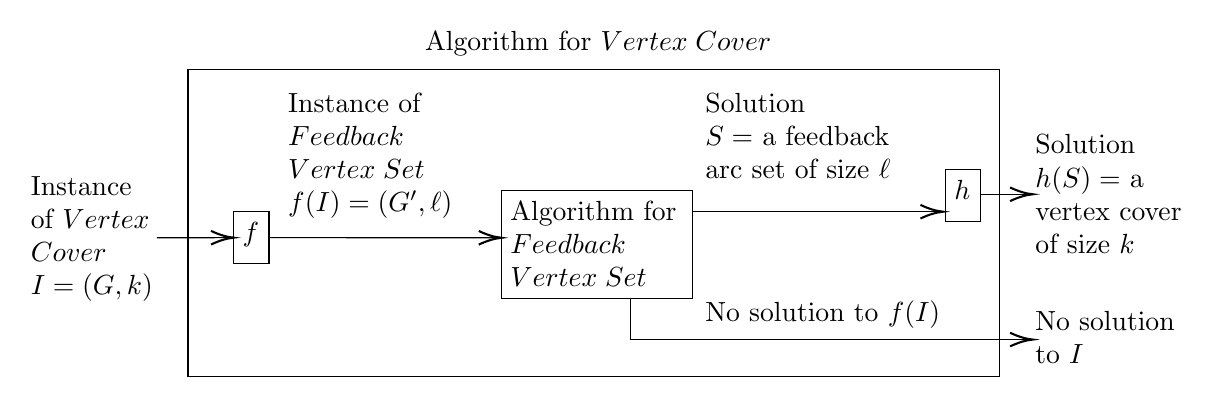
\begin{tikzpicture}[x=0.75pt,y=0.75pt,yscale=-1,xscale=1]
%uncomment if require: \path (0,300); %set diagram left start at 0, and has height of 300

%Shape: Rectangle [id:dp05068879160984241] 
\draw   (87,70) -- (478,70) -- (478,217.9) -- (87,217.9) -- cycle ;
%Straight Lines [id:da16135743905999322] 
\draw    (330,138.4) -- (450.8,138.4) ;
\draw [shift={(450.8,138.4)}, rotate = 180] [color={rgb, 255:red, 0; green, 0; blue, 0 }  ][line width=0.75]    (10.93,-3.29) .. controls (6.95,-1.4) and (3.31,-0.3) .. (0,0) .. controls (3.31,0.3) and (6.95,1.4) .. (10.93,3.29)   ;
%Straight Lines [id:da7113802494602071] 
\draw    (300,180) -- (300,200) ;
%Straight Lines [id:da39032910531245935] 
\draw    (300,200) -- (494,200) ;
\draw [shift={(494,200)}, rotate = 180] [color={rgb, 255:red, 0; green, 0; blue, 0 }  ][line width=0.75]    (10.93,-3.29) .. controls (6.95,-1.4) and (3.31,-0.3) .. (0,0) .. controls (3.31,0.3) and (6.95,1.4) .. (10.93,3.29)   ;
%Straight Lines [id:da5950145693340629] 
\draw    (469,130) -- (494,130) ;
\draw [shift={(494,130)}, rotate = 180] [color={rgb, 255:red, 0; green, 0; blue, 0 }  ][line width=0.75]    (10.93,-3.29) .. controls (6.95,-1.4) and (3.31,-0.3) .. (0,0) .. controls (3.31,0.3) and (6.95,1.4) .. (10.93,3.29)   ;

% Text Node
\draw (200,50) node [anchor=north west][inner sep=0.75pt]   [align=left] {Algorithm for $Vertex\;Cover$};
% Text Node
\draw (10,120) node [anchor=north west][inner sep=0.75pt]   [align=left] {Instance\\of $Vertex$\\$Cover$\\$I = (G,k)$};
% Text Node
\draw    (109,138.4) -- (126,138.4) -- (126,163.4) -- (109,163.4) -- cycle  ;
\draw (112,142.4) node [anchor=north west][inner sep=0.75pt]   [align=left] {$f$};
% Text Node
\draw (134,80) node [anchor=north west][inner sep=0.75pt]   [align=left] {Instance of\\$Feedback$ \\$Vertex\;Set$\\$f(I) = (G^\prime,\ell)$};
% Text Node
\draw    (238,128) -- (330,128) -- (330,180) -- (238,180) -- cycle  ;
\draw (241,132) node [anchor=north west][inner sep=0.75pt]   [align=left] {Algorithm for\\$Feedback$ \\$Vertex\;Set$};
% Text Node
\draw (335,80) node [anchor=north west][inner sep=0.75pt]   [align=left] {Solution\\$S = $ a feedback\\arc set of size $\ell$};
% Text Node
\draw    (452,118) -- (469,118) -- (469,143) -- (452,143) -- cycle  ;
\draw (455,122) node [anchor=north west][inner sep=0.75pt]   [align=left] {$h$};
% Text Node
\draw (494,185) node [anchor=north west][inner sep=0.75pt]   [align=left] {No solution\\to $I$};
% Text Node
\draw (335,180) node [anchor=north west][inner sep=0.75pt]   [align=left] {No solution to $f(I)$};
% Text Node
\draw (494,100) node [anchor=north west][inner sep=0.75pt]   [align=left] {Solution\\$h(S) = $ a\\vertex cover\\of size $k$};
% Connection
\draw    (126,150.9) -- (236,150.96) ;
\draw [shift={(238,150.97)}, rotate = 180.03] [color={rgb, 255:red, 0; green, 0; blue, 0 }  ][line width=0.75]    (10.93,-3.29) .. controls (6.95,-1.4) and (3.31,-0.3) .. (0,0) .. controls (3.31,0.3) and (6.95,1.4) .. (10.93,3.29)   ;
% Connection
\draw    (72,150.96) -- (107,150.91) ;
\draw [shift={(109,150.91)}, rotate = 539.9300000000001] [color={rgb, 255:red, 0; green, 0; blue, 0 }  ][line width=0.75]    (10.93,-3.29) .. controls (6.95,-1.4) and (3.31,-0.3) .. (0,0) .. controls (3.31,0.3) and (6.95,1.4) .. (10.93,3.29)   ;

\end{tikzpicture}











An instance of Vertex Cover is a graph $G = (V,E)$ and a positive integer $k$. We need to transform this into an instance for Feedback Arc Set: a graph $G^\prime = (V^\prime , E^\prime)$\footnote{The superscripts `*' and `$\prime$' mean different things in different sections of this paper.} and a positive integer $\ell$.

\begin{itemize}
    \item $f((G = (V,E),k)) = (G^\prime = (V^\prime , E^\prime), \ell)$ where the peculiarities of $G^\prime$ are:
    \begin{itemize}
        \item For each vertex $v$ in $V$, there are two vertices $x_v$ and $y_v$ in $V^\prime$.
        \item Moreover, each pair of vertices $x_v$ and $y_v$ is connected by a directed edge $(x_v,y_v)$. 
        \item For each edge $(u,v)$ in $E$, there are two directed edges $(y_u,x_v)$ and $(y_v,x_u)$.
        \item Consequently, if $|V| = n$ then $|V^\prime| = 2n$ and $|E^\prime| = n + 2|E|$.
    \end{itemize}
    \item Finally, $k = \ell$.
\end{itemize}

Now, suppose we have a solution, $S$, to FeedBack Arc Set for $(G^\prime,\ell)$, then we will return the set comprising of each edge $e=(x_u,y_u) \in S$ corresponding to each vertex $u$ in $h(S) = S^*$.

\begin{itemize}
    \item $h(S) = S^* = \{u \in V\;|\;(x_u,y_u) \in S\}$
\end{itemize}
    
This reduction will be correct if the following theorem is true:

\begin{theorem}
    $S$ is a feedback arc set on $G^\prime = (V^\prime,E^\prime)$ of size $\ell$ if and only if $h(S) = S^*$ is a vertex cover on $G = (V,E)$ of size $\ell$.~\cite{upenn2003}~\cite{toronto2014}
\end{theorem}
    
\begin{proof}

($\Rightarrow$) Suppose $S$ is a feedback arc set on $G^\prime = (V^\prime,E^\prime)$ and $|S|=\ell$. Without loss of generality we can assume
that the only edges that may be removed from $E^\prime$ to make the resulting graph $G^* = (V^\prime,E^\prime-S)$ a DAG (i.e., all the edges in $S$) are of the form $(x_u, y_u)$. Because if some other edge $(y_u, x_v)$ were to have been removed, all cycles in which this edge participated would have included $(x_v,y_v)$, say, and this edge could have been removed instead. The set $S^* = \{u \in V\;|\;(x_u,y_u) \in S\}$ would then form a vertex cover. Further, for a contradiction, suppose that $S^*$ ($|S^*|=\ell$) is not a node cover on $G = (V,E)$. Since $S$ is not a node cover on $G$, there must exist some edge, $e=(u,v)\in E$ such that it is not covered by $S^*$. Then, in $G^\prime$ the cycle $(x_u, y_u)$, $(y_u, x_v)$, $(x_v, y_v)$, $(y_v, x_u)$ is unbroken
by the removal of all the edges in $S$. Therefore $S$ would not be a feedback arc set on $G^\prime$. $\rightarrow \leftarrow$.

($\Leftarrow$) Suppose $S^*$ is a vertex cover on $G = (V,E)$ and $|S^*|=\ell$. Now, suppose for each vertex $v\in S^*$ we pick the edge $(x_v,y_v)$ from $G^\prime$ and build the set $S$ out of these chosen edges, then the graph $G^* = (V^\prime,E^\prime \setminus S)$ will be a DAG and thus $S$ will be a feedback arc set on $G^\prime$. But, for a contradiction, suppose that $G^*$ (which will of course have $|E^\prime| - \ell$ edges) is not a DAG. Going back to $G^\prime$, if a directed cycle enters a vertex $x_u$ it can only leave by the edge $(x_u, y_u)$. Similarly, a cycle can only enter $y_u$ through the edge $(x_u, y_u)$. Thus if a cycle in $G^\prime$ uses the edge $(y_u, x_v)$ it must also use the edges $(x_u, y_u)$ and $(x_v, y_v)$. But at least one of $(x_u, y_u)$ or $(x_v, y_v)$ should have been removed in $G^*$ as per our construction of $G^*$ and if $S^*$ were truly a vertex cover i.e., a set of vertices that includes at least one endpoint of every edge of the graph. And, since the only cycles possible in $G^*$ are each of the cycles involving the sets of topologically adjacent vertices $x_u, y_u, x_v, y_v$ and since there should at least be one cycle in $G^*$ for it to not be a DAG, it should be the case that at least one of the edges $(u,v) \in E$ is not covered by $S^*$. Therefore $S^*$ is not a node cover. $\rightarrow \leftarrow$. 
\end{proof}

\section{Brute Force Algorithm}

 \begin{algorithm}[H]
  \caption*{{\sc BruteForceFeedbackArcSet($G=(V,E),k$)}}
  \begin{algorithmic}[1]
\INPUT A graph $G = (V,E)$ and a positive integer $k$

\OUTPUT A set of $k$ edges, $S$, that form a feedback arc set, or a statement that no such feedback arc set exists.


\For{all subsets $R\subseteq E$ of size $k$}
\If {$R$ is a feedback arc set}
\State {return $R$}
\EndIf
\EndFor
\State {return ``no such feedback arc set"}

  
  \end{algorithmic}
  \end{algorithm}
  
The algorithm considers all possible subsets of $|E|=m$ edges of size $k$, there are $m \choose k$ of these sets. For each of these subsets, $R$, {\sc BruteForceFeedbackArcSet} checks if $R$ is a feedback arc set (this can be done using topological sort in time $O(m + n)$ where $|V| = n$). Thus, the total running time is $O((m + n){m\choose k})$. 

\section{Approximation Algorithm}

In order to use an approximation ratio, it is easier to consider approximating a weighted digraph version of FAS. Here we give a $\lambda$-approximation algorithm for the optimization version of feedback arc set where $\lambda$ is the length, in terms of number of arcs, of a longest simple cycle of the digraph.~\cite{demetrescu_combinatorial_2003-1} Note that the length is in terms of number of arcs, and therefore independent of the weight function.

The minimum FAS problem consists of finding a smallest cost feedback arc set where the cost of the feedback set can be either its cardinality or its weight with respect to a nonnegative weight function. Here is the modified optimization problem:

\vspace{.5cm}
\noindent\fbox{
\parbox{\textwidth}{
{\bf Weighted Feedback Arc Set}

    {\bf Input:} A digraph $G = (V,E)$ with nonnegative arc weights $w: E\rightarrow \mathbb{R^+}$

    {\bf Goal:} Return a minimum weight arc set $S\subseteq E$ such that the directed graph $(V,E\setminus S)$ is acyclic
}
}
\vspace{.5cm}

\begin{itemize}
    \item Let the weight of a feedback arc set $S$ be denoted by $w(S) = \sum_{(x,y)\in E} w(x,y)$.
    \item A feedback arc set $S^*$ is optimum if $w(S^*) \leq w(S^\prime)$ for any feedback arc set $S^\prime$.
    \item A feedback arc set $S^\prime$ is a $r$-approximation with $r \geq 1$, if $w(S^\prime) \leq r\cdot w(S^*)$.
\end{itemize}

The Weighted Feedback Arc Set problem is the problem of covering all cycles of a given digraph by means of a minimum cost set of arcs. In that case, the following theorem will come in handy:

\begin{theorem}
    Local Ratio Theorem: If a cover $C$ is a $r$-approximation with respect to both a weight function $w_1$ and a weight function $w_2$, then $C$ is an $r$-approximation with respect to the weight function $w_1 + w_2$.
\end{theorem}

In other words, if the payment at each step can be proved to cost no more than $r$ times the optimal payment, then the total payment will be at most $r$ times the optimal cost. Following this approach we may progressively reduce the weights of the arcs of the digraph and add to the FAS the arcs whose weight becomes 0.

  \vspace{.5cm}
Consider the following algorithm:

 \begin{algorithm}[H]
  \caption*{{\sc WeightedFeedbackArcSetApproximation($G=(V,E), w: E\rightarrow \mathbb{R^+}$)}}
  \begin{algorithmic}[1]
\INPUT A digraph $G$ and a nonegative weight function $w$. 

\OUTPUT A feedback arc set $S$ of minimal weight.

\State {$S = \emptyset$}
\While {$(V,E\setminus S)$ is not acyclic} \Comment{Phase 1}
\State Let $\mathcal{C}$ be a simple cycle in $(V,E\setminus S)$
\State Let $(x,y)$ be a minimum weight arc in $\mathcal{C}$ and let $\varepsilon$ be its weight
    \For {all $(u,v)\in \mathcal{C}$}
    \State $w(u,v) = w(u,v) - \varepsilon$
    \If {$w(u,v) = 0$}
        \State $S = S \cup \{(u,v)\}$
    \EndIf
    \EndFor
\EndWhile

\For {all $(u,v)\in S$} \Comment{Phase 2}
    \If {$(V,(E\setminus S) \cup \{(u,v)\})$ is acyclic}
    \State $S = S\setminus \{(u,v)\}$
    \EndIf
\EndFor
\State Return S

\end{algorithmic}
\end{algorithm} 

\subsection{Algorithmic Analysis}

\paragraph{Intuition:} The algorithm consists of two phases. First, it looks for a simple cycle $\mathcal{C}$ in the digraph. If such a cycle exists, it identifies an arc in $\mathcal{C}$ having minimum weight, say $\varepsilon$. Then, the weight of all the arcs in $\mathcal{C}$ is decreased by $\varepsilon$ and the arcs
whose weights become 0 are removed. If the digraph is now acyclic the first phase terminates, otherwise it is repeated.

After Phase 1, the set of deleted arcs is certainly a feedback arc set, though not necessarily minimal. Hence, the algorithm tries to add back to the digraph some of the deleted arcs, taking care not to re-introduce cycles. The set of removed arcs is finally returned. All these steps are demonstrated in figure~\ref{fig:my_fig}.

{\sc WeightedFeedbackArcSetApproximation} roughly tries to find a compromise between two (somewhat opposite) approaches, i.e., removing light arcs, that is, arcs with small weight, and removing arcs belonging to a large number of cycles. Light arcs are convenient to be deleted as they contribute to breaking cycles, yet increasing the weight of the feedback set only to a limited extent. On the other hand, if a heavy arc belongs to a large number of cycles, it may be convenient to choose it instead of a numerous set of light arcs.

\begin{figure}[H]
    \centering
    \includegraphics[scale=0.5]{figures/fas-steps.png}
    \caption{An illustration of {\sc WeightedFeedbackArcSetApproximation}}
    \label{fig:my_fig}
\end{figure}

\begin{itemize}
    \item Is the algorithm {\em feasible}? Does it return a feedback arc set?
    \item How close is the size of the feedback arc set that the algorithm gives to the size of the optimal FAS?
\end{itemize}

We'll answer the question of feasibility first:

\begin{theorem}
    Let $G = (V, E, w)$ be a weighted directed graph with $n$ vertices and $m$
arcs. {\sc WeightedFeedbackArcSetApproximation} finds a minimal feedback arc set of $G$ in $O(m\cdot (m+n))$ worst-case running time.  
\end{theorem}

\begin{proof}
\paragraph{Correctness:}
{\sc WeightedFeedbackArcSetApproximation} progressively removes arcs from the input digraph, stopping only when the remaining arcs do not form cycles (lines 2-8). Hence, the set of arcs removed after the first phase is by definition a feedback arc set. To guarantee the minimality of the solution, a maximal subset of the previously removed arcs is added back in the second phase (lines 9-11): in this phase $S$ remains a feedback arc set because the acyclicity condition is tested before any arc addition (line 10).

\paragraph{Runing Time:} At most $m$ iterations can be done in the first phase, since at each step at least one arc is removed from the digraph (i.e., a minimum weight arc in $\mathcal{C}$). At each iteration three basic operations are performed: a simple cycle is found (line 3), a minimum weight arc in the cycle is identified (line 4), and the weights of all arcs in the cycle are updated (lines 5-8). The second and third operations can be performed in $O(n)$ time, as $n$ is the maximum length of any simple cycle of $G$. A straight-forward implementation of the first operation (by means of a visit), would yield $O(m\cdot (m+n))$ overall running time.
\end{proof}
  \vspace{.5cm}

Now we will show that {\sc WeightedFeedbackArcSetApproximation} gives a $\lambda$-approximation for feedback arc set.

We denote with $w, w_1, w_2$ different nonnegative weight functions for the arcs of a digraph $G = (V, E)$. Moreover, let $S^*, S_1^*, S_2^*$ be the minimum
feedback arc sets of the weighted digraphs $(V, E, w), (V, E, w_1), (V, E, w_2)$ respectively. The following lemma relates the values of the weights of the minimum feedback arc sets with respect to different weight functions $w, w_1, w_2$ when these functions are linearly dependent:

\begin{lemma}
    Let $G = (V, E)$ be a directed graph and let $w, w_1, w_2$ be three nonnegative weight functions on the arcs of $G$ such that $w = w_1 + w_2$. Then it holds: $$w_1(S_1^*) + w_2(S_2^*) \leq w(S^*)$$
\end{lemma}

\begin{proof}
    Since $w = w_1 + w_2$, we have that $w(S^*) = w_1(S^*) + w_2(S^*)$. Moreover, $S^*$ is a feedback arc set for $G$ with respect to both $w_1$ and $w_2$, but it is not necessarily a minimum feedback arc set. Hence, we have that $w_1(S^*) \geq w_1(S_1^*)$ and $w_2(S^*) \geq w_2(S_2^*)$. The claim immediately follows.
\end{proof}

\begin{theorem}
    Let $G = (V, E, w)$ be a weighted directed graph. {\sc WeightedFeedbackArcSetApproximation} approximates a minimum feedback arc set of $G$ within a ratio bounded by the length $\lambda$ of a longest simple cycle of $G$.
\end{theorem}

\begin{proof}
    The second phase of {\sc WeightedFeedbackArcSetApproximation} is only required for making the previously found feedback arc set minimal. Since the weight of the feedback arc set can only decrease during this phase, it is sufficient to prove that the approximation ratio is already guaranteed after Phase 1. The proof proceeds by induction on the number of iterations of the while-loop in line 2 of the algorithm. This number is finite and strictly decreasing since at each step at least one arc is removed from the digraph.
    
    \paragraph{Base step:} No iteration is performed. In this case the input digraph is already acyclic and the empty feedback arc set is obviously an optimal solution.
    
    \paragraph{Induction step:} Let us consider a generic iteration of the algorithm and let us denote with $w$ the weight of the arcs of $G$ in that iteration. Let $\mathcal{C}$ be the simple cycle identified by the algorithm (line 3), let $k$ be its length, and let $\varepsilon$ be the weight of the smallest cost arc in $\mathcal{C}$. We define a new weight function $w_1$ for the digraph $G = (V, E)$ as follows:
    
    \begin{equation*}
    \forall (u,v) \in E, 
    w_1(u,v) = \begin{cases}
               \varepsilon          & if\;(u,v) \in \mathcal{C}\\
               0                    & \text{otherwise}
           \end{cases}
    \end{equation*}
    
    Observe that the cost of the minimum feedback arc set of the digraph $G = (V, E)$ with respect to $w_1$ is equal to $\varepsilon$, i.e., $w_1(S_1^*) = \varepsilon$: this is because cycle $\mathcal{C}$ is simple, and removing only one arc is sufficient to break it.
    
    Moreover, the weight of any feedback arc set $S$ w.r.t $w_1$ cannot be greater than $k\cdot \varepsilon \leq \lambda \cdot \varepsilon$, because all the arcs not belonging to $\mathcal{C}$ cost 0 and at most all the arcs in $\mathcal{C}$ can participate to $S$. Therefore, for any $S$:
    
    $$w_1(S) \leq \lambda \cdot w_1(S_1^*)$$

    In the following we denote with $S_1$ the set of arcs of cycle $\mathcal{C}$ removed by the algorithm in order to break it. As far as the algorithm is concerned, $S_1 = \{(u,v) \in \mathcal{C}\;such\;that\; w(u,v) = \varepsilon\}$. Since any arc $(u,v) \in \mathcal{C}$ has weight $w_1(u,v)$ equal to $\varepsilon$, it holds:
    
    $$w(S_1) = w_1(S_1)$$
    
    Let us now define a new weight function $w_2 = w-w_1$. We have that $0 \leq w_2(\cdot) \leq w(\cdot)$ since $w(\cdot) \geq w_1(\cdot) \geq 0$. In addition, by the inductive hypothesis on the digraph $(V, E\setminus S_1, w_2)$, {\sc WeightedFeedbackArcSetApproximation} returns a feedback arc set $S_2$ of this digraph such that: $$w_2(S_2) \leq \lambda \cdot w_2(S_2^*)$$.
    
    Let $S$ be the feedback arc set returned by {\sc WeightedFeedbackArcSetApproximation} on the weighted digraph $G = (V, E, w)$. As far as the algorithm is concerned, $S$ consists both of the arcs in $S_1$ and of the arcs in $S_2$, i.e., $S = S_1 \cup S_2$. It is also worth pointing out that $S_1 \cap S_2 = \emptyset$, due to the fact that once an arc has been removed, it will be no longer be considered by the algorithm. By linearity of $w, w_1, w_2$, it holds $w(S) = w_1(S) + w_2(S)$. In conclusion:
    \newpage
    $$w(S) =$$ 
    \Comment{$w = w_1 + w_2$}
    $$w_1(S) + w_2(S) =$$
    \Comment{$S = S_1 \cup S_2$}
    $$w_1(S) + w_2(S_1) + w_2(S_2) - w_2(S1 \cap S2) =$$
    \Comment{$S_1 \cap S_2 = \emptyset$}
    $$w_1(S) + w_2(S_1) + w_2(S_2) =$$
    \Comment{$w_2 = w-w_1$ and $w(S_1) = w_1(S_1)$}
    $$w_1(S) + w_2(S_2) \leq$$
    \Comment{$w_1(S) \leq \lambda \cdot w_1(S_1^*)$}
    $$\lambda \cdot w_1(S_1^*) + w_2(S_2) \leq$$
    \Comment{Inductive Hypothesis}
    $$\lambda \cdot w_1(S_1^*) + \lambda \cdot w_2(S_2^*) \leq$$
    \Comment{Lemma 6}
    $$\lambda \cdot w(S^*)$$

    
    The inequality $w(S) \leq \lambda \cdot w(S^*)$ proves that {\sc WeightedFeedbackArcSetApproximation} is a $\lambda$-approximation algorithm.

\end{proof}

\section{Applications/Other Interesting Things}

\begin{itemize}
    \item There are several practical applications of FAS including the analysis of large-scale systems with feedback, graph layout~\cite{sugiyama_methods_1981}, and certain scheduling problems~\cite{flood_exact_1990}.
    \item The minimum feedback arc set problem on undirected graphs can be easily solved in polynomial time by finding a maximum weight spanning tree. Moreover, although its directed version is NP-complete even on digraphs with total vertex in-degree and out-degree smaller than 3, yet it is polynomial-time solvable on planar digraphs~\cite{lucchesi_minimax_1978}.
\end{itemize}

\bibliographystyle{plain}
\bibliography{references.bib}

\end{document}
